\documentclass[12pt]{article}

% \usepackage{extsizes}  % 字體文件使用 14pt
\usepackage{CJKutf8}
\usepackage[margin=2.0cm]{geometry}
\usepackage{fancyhdr}  % 頁首、頁尾
\usepackage{graphicx}
\usepackage{amsmath, amssymb, amsfonts}
\usepackage{listings}  % code showing
\usepackage{pagecolor}  % for code color define
\usepackage{tocloft}  % contents
\usepackage{float} %设置图片浮动位置的宏包
\usepackage{blkarray, bigstrut}
\usepackage{hyperref}
\numberwithin{figure}{section}
\numberwithin{table}{section}
\numberwithin{equation}{section}

% -- 格式
\pagestyle{fancy}  % 使用 header
\fancyhf{}
\setcounter{secnumdepth}{6}  % 移除 section 數字
\renewcommand{\cftsecleader}{\cftdotfill{\cftdotsep}}

%----------- watermark -----------
\usepackage{wallpaper}
\CenterWallPaper{0.174}{watermark.jpg}
\setlength{\wpXoffset}{6.1725cm}
\setlength{\wpYoffset}{10.5225cm}


\title{{$~~~$國立臺灣大學工學院機械工程學系
\newline $~~~~$Department of Mechanical Engineering
\newline $~~~~~~~~~$College of Engineering
\newline $~~~~~~~~$National Taiwan University
\newline 
\newline 
\newline $~~~~~~~~~~~$Orientation Homework
\newline 
\newline 
\newline 
\newline R10522614 賴重叡}}
\date{}
\author{}


%% -- 標題使用中文取代
\renewcommand{\figurename}{圖}
\renewcommand{\tablename}{表}
\renewcommand{\lstlistingname}{程式碼}



%% -- 間距設定
 \linespread{1.5}\selectfont  % 行距
\setlength{\headheight}{29pt}
\setlength\parindent{0pt}
\setlength{\parskip}{0.5em}
\setlength{\abovecaptionskip}{10pt}  % 圖表標題 caption 與圖表的距離
\setlength{\belowcaptionskip}{10pt}

% -- 顯示程式碼格式
\definecolor{codegreen}{rgb}{0,0.6,0}
\definecolor{codegray}{rgb}{0.5,0.5,0.5}
\definecolor{codepurple}{rgb}{0.58,0,0.82}
\definecolor{backcolour}{rgb}{0.95,0.95,0.92}
\lstdefinestyle{pystyle}{
    backgroundcolor=\color{backcolour},
    commentstyle=\color{codegreen},
    keywordstyle=\color{magenta},
    numberstyle=\footnotesize\color{codegray},
    stringstyle=\color{codepurple},
    basicstyle=\ttfamily\footnotesize,
    breakatwhitespace=false,
    breaklines=true,
    captionpos=b,
    keepspaces=true,
    numbers=left,
    numbersep=5pt,
    showspaces=false,
    showstringspaces=false,
    showtabs=false,
    tabsize=2,
    extendedchars=false
}
\lstset{style=pystyle}
% ---------------------------------------------

\begin{document}
\begin{CJK}{UTF8}{bkai}

\chead{\normalsize \textbf{Homework}}  % 可調整大小
\lhead{\normalsize Orientation}
\rhead{\normalsize R10522614 賴重叡}
\cfoot{\thepage}


\maketitle
\thispagestyle{empty}
\begin{center}
\vfill
{\large \today}
\end{center}

\newpage
\tableofcontents\thispagestyle{fancy}
\thispagestyle{empty}



% ---------------------------------------------
\newpage
\setcounter{page}{1}
\section{Problem sheet}

\begin{figure}[H] 
    \centering 
    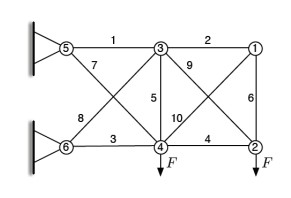
\includegraphics[width=0.5\textwidth]{1-1.jpg} 
    \caption{十桿桁架結構示意圖} 
    \label{Fig.1-1} 
\end{figure}
十桿桁架(ten-bar truss)是典型的桁架結構之一,如圖 \ref{Fig.1-1} 所示。此作業以二維的十桿桁架為題,藉由有限元素法(finite element method,FEM)將每一桿件視為個別的元素,計算其受外力的反應,並在符合條件的情況下做出輕量化。

\subsection{Problem Definition}
在以下已知條件下,給定桿件截面半徑,求各桿件的位移、應力與反作用力,並進行最佳化:
\begin{itemize}
    \item 整體架構處在靜力平衡的情況下;
    \item 所有桿件截面皆為圓形;
    \item 材料為鋼,楊氏係數 $E = 200 GPa$,密度 $\rho  = 7860 kg/m^3$,降伏強度 $\sigma _y = 250 MPa$;
    \item 平行桿件與鉛直桿件(桿件1至桿件6)長度皆為 9.14 m;
    \item 桿件 1 至桿件 6 截面半徑相同為 $r_1$,桿件 7 至桿件 10 截面半徑相同為 $r_2$;
    \item 所有桿件半徑的最佳化範圍為 0.001 至 0.5 m 之間;
    \item 在節點 2 和節點 4 上的負載 F 皆為 $1.0 × 10^7$ N 向下。
\end{itemize}


\subsection{objective function}

\begin{equation}
    \label{obj_fun}
    \min_{r_1,r_2}  f(r_1,r_2)  = \sum_{i=1}^{6} m_i(r_1)+\sum_{i=7}^{10} m_i(r_2) 
\end{equation}

\begin{eqnarray*}    \label{eq}
    subject\ to   & & \left\lvert \boldsymbol{\sigma_i}\right\rvert \leqq \sigma_y    \\
                  & &\Delta s_2\leqq 0.02    \\
    where         & &f : \text {所有桿件的質量}    \\
                  & &\Delta s_2: \text {node 2 的位移} \\
                  & &\sigma _y: \text{降伏應力} \\
                  & &\boldsymbol{\sigma_i}: \text{所有桿件的應力}
\end{eqnarray*}


\clearpage
\section{Theoretical formulation and Code}

\subsection{Truss}

定義上,桁架(truss)是以多個長桿由端點互相連接而成的結構,因為桿件的數量和尺寸等規格皆可以變動,可以組合出的幾何型態更是非常多變,很容易適用於各種工程應用的場域,因此桁架工程應用甚廣,是房屋、橋梁等建築非常常見的結構。

處理桁架問題時所套用的物理模型,通常使用以下假設:
\begin{itemize}
    \item 外力與內力均作用於桿件端點上;
    \item 各桿件間的連接簡化為銷釘連接(pin connection);
    \item 忽略桿件本身重量之影響,因此各桿件視為二力構件(two-force member);
    \item 定義各桿件之受力正方向為拉伸,負方向為壓縮。
\end{itemize}



\subsection{Trusses Using FEA and Code}
在本節中,將應用有限元素法來解二維桁架的問題。 該方法比最初用於解決桁架問題的方法稍微複雜一些,但其可以解決涉及靜不定結構的問題。各桿件視為元素(element)、元素間的連接為節點(node),求解流程如\ref{Fig.2-1}。首先建立元素表格(element table),利用表格中的資料計算出剛性矩陣(stiffness matrix),再以力、剛性和位移三者之間的關係找出所求的位移,最後應力和反作用力也能透過位移計算而得。
\begin{figure}[H] %H为当前位置,!htb为忽略美学标准,htbp为浮动图形
    \centering %图片居中
    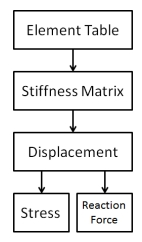
\includegraphics[width=0.2\textwidth]{2-1.jpg} %插入图片,[]中设置图片大小,{}中是图片文件名
    \caption{十桿桁架有限元素法流程} %最终文档中希望显示的图片标题
    \label{Fig.2-1} %用于文内引用的标签
\end{figure}

\begin{description}
	\item [Step 1] Element Table\\
		將各元素和節點編號後 (本節以圖 \ref{Fig.1-1} 中的編號為主),先記錄各節點的座標,方便計算元素表格使用(如表 \ref{nodeCoor}):

		\begin{table}[h]
		\caption{節點座標}
		\label{nodeCoor}
		\renewcommand{\arraystretch}{1.1}
		\centering
		\begin{tabular}{ccc}
		\hline
		\makebox[2.5cm]{node} & \makebox[2cm]{$x$} & \makebox[2cm]{$y$} \\
		\hline
		1   &18.28 & 9.14 \\
		2   &18.28 & 0 \\
		3   & 9.14  & 9.14 \\
		4   &9.14  & 0 \\
		5   & 0   &9.14 \\
		6   & 0   & 0 \\
		\hline
		\end{tabular}
		\end{table}
        ~\\
		首先在表格中填入各元素兩端的節點,再計算面積、長度、角度等資料(如表 \ref{elementTable}):

		\begin{table}[h]
		\caption{元素表格}
		\label{elementTable}
		\renewcommand{\arraystretch}{1.1}
		\centering
		\begin{tabular}[c]{cccccccc}
		\hline
		\makebox[1.8cm]{Element} & \makebox[1.3cm]{node $i$} & \makebox[1.3cm]{node $j$} & \makebox[0.5cm]{E}& \makebox[0.5cm]{A}& \makebox[0.7cm]{$L$}& \makebox[0.7cm]{$\cos$}& \makebox[0.7cm]{$\sin$}\\
		\hline
		{\bf1}   & 3   & 5 \\
		{\bf2}   & 1   & 3 \\
		{\bf3}   & 4   & 6 \\
		{\bf4}   & 2   & 4 \\
		{\bf5}   & 3   & 4 \\
		{\bf6}   & 1   & 2 \\
		{\bf7}   & 4   & 5 \\
		{\bf8}   & 3   & 6 \\
		{\bf9}   & 2   & 3 \\
		{\bf10}   & 1   & 4 \\
		\hline
		\end{tabular}
		\end{table}

		彈性係數 $E$ 為題目已知,截面積以半徑 $r_1$ 或 $r_2$ 透過圓面積公式計算:
		\begin{equation}
		    \label{eq_cirArea}
		    A=\pi r^2
		\end{equation}

		利用各元素兩端的節點座標,以畢氏定理計算出桿長:
		\begin{equation}
		    \label{eq_lenth}
		    L=\sqrt{(x_{\mathrm{node\, j}}-x_{\mathrm{node\,i}})^2+(y_{\mathrm{node\,j}}-y_{\mathrm{node\,i}})^2}
		\end{equation}

		以長度除兩端節點的 $x$ 座標變量即角度的 $\cos$ 值,除 $y$ 座標變量即角度的 $\sin$ 值:
		\begin{align}
		\label{eq_cos}
		\cos \theta_e=\frac{(x_{\mathrm{node\,j}}-x_{\mathrm{node\,i}})}{L}\\
		\label{eq_sin}
		\sin \theta_e=\frac{( \mathrm{y_{node\,j}}-y_{ \mathrm{node\,i}})}{L}
		\end{align}

		將式 \ref{eq_cirArea} 至 \ref{eq_sin} 計算出所有元素的規格和位置統整至表 \ref{elementTable},便可得到完整的元素表格,此表囊括下一步驟計算剛性矩陣所需的所有數據。此步驟的程式,如程式碼 \ref{FEA1}。\\

        \lstinputlisting[
            language=MATLAB, firstline=2, lastline=19, firstnumber=1,
            caption={Step1程式(by Matlab)}, label={FEA1}
        ]{./FEA.m}

	\item [Step 2] Stiffness Matrix\\
		每個元素末端連接兩個節點,節點又分別有 $x$ 和 $y$ 兩個方向的自由度 (degree of freedom,DOF),以 $4\times4$ 的剛性矩陣 (stiffness matrix,數學式中以 ${\bf k}$ 表示) 表示元素中4個自由度上位移和受力之間的相互關係:
		\begin{equation}
		\label{eq_kMatrix}
		{\bf k}^e=\frac{EA_e}{L_e}
		\left[
		\begin{array}{cccc}
		c^2 & cs & -c^2 & -cs\\
		cs & s^2 & -cs &-s^2\\
		-c^2 & -cs & c^2 & cs\\
		-cs & -s^2 & cs & s^2
		\end{array}
		\right]
		\end{equation}
		其中 $c$ 表示 $\cos \theta_e$;$s$ 表示 $\sin \theta_e$。

		桁架整體結構中有 6 個節點,總共有 $2\times6=12$ 個自由度,以 node1 在 $x$ 方向為 DOF1、 node1 在 $y$ 方向為 DOF2、node2 的 $x$ 方向為 DOF3......依 node1 到 node6 的順序和 $x$、$y$ 的順序編號 12 個自由度。透過元素表格揭露的數據代入式 \ref{eq_kMatrix} ,建立各元素的剛性舉陣。


		10 個元素皆參考元素表格代入式 \ref{eq_kMatrix}  推導出剛性矩陣後,按照所對應的自由度,整合成 $12\times12$ 的整體剛性矩陣 $\textbf{K}$ ( 式 \ref{eq_KMatrix} ):
		\begin{equation}
		\label{eq_KMatrix}
		\textbf{K}\leftarrow \sum_{e} \textbf{k}^e\\
		\end{equation}

        此步驟的程式,如程式碼 \ref{FEA2}。\\
        \lstinputlisting[
            language=MATLAB, firstline=23, lastline=63, firstnumber=19,
            caption={Step2程式(by Matlab)}, label={FEA2}
        ]{./FEA.m}

	\item [Step 3] Displacement\\
		為了利用力、剛性和位移三者之間的關係:
		\begin{equation}
			\label{eq_F=KQ}
			{\bf F}={\bf K}{\bf Q}
		\end{equation}
		承 Step2 設定整體系統的 12 個自由度,建立對應 12 個自由度的 $12\times1$ 力向量和 $12\times1$ 位移向量。
		\begin{align}
		\label{eq_forceVector}
			\textbf{F}&= \:\,
			\left[
			\begin{array}{cccc}
			F_1 & F_2 & ... & F_{12}
			\end{array}
			\right]^T\\
		\label{eq_displacementVector}
			\textbf{Q}&= \:\,
			\left[
			\begin{array}{cccc}
			Q_1 & Q_2 & ... & Q_{12}
			\end{array}
			\right]^T
		\end{align}

		套用邊界條件,node5 和 node6 為固定端,在 $x$、$y$ 方向均無位移:
		\begin{equation}
		\label{eq_boundaryConditions}
		Q_9 = Q_{10} = Q_{11} = Q_{12} = 0
		\end{equation}
		由於 DOF9 至 DOF12 無位移,可以將剛性矩陣 $\textbf{K}$、力向量 $\textbf{F}$、位移向量 $\textbf{Q}$ 中相對應的行與列消除。剛性矩陣 $\textbf{K}$ 截取第 1 行到第 8 行、第 1 列到第 8 列,簡化成 $8\times8$ 的 $\textbf{K}_{reduced}$;力向量 $\textbf{F}$ 和移向量 $\textbf{Q}$ 簡也只取前 8 個,化簡成 $8\times1$ 的 $\textbf{F}_{reduced}$ 和 $\textbf{Q}_{reduced}$:

		\begin{align}
		\label{eq_kReaction}
			{\bf K}_{\mathrm{reduced}}&=
			\left[
			\begin{array}{cccc}
			K_{1,1} & K_{1,2} & \cdots &K_{1,8}\\
			K_{2,1} & K_{2,2} & \cdots &K_{2,8}\\
			\vdots & \vdots &  \ddots&\vdots\\
			K_{4,1} & K_{8,2} & \cdots &K_{8,8}\\
			\end{array}
			\right]\\
		\label{eq_reducedForceVector}
			\textbf{F}_{\mathrm{reduced}}&= \:\,
			\left[
			\begin{array}{cccc}
			F_1 & F_2 & ... & F_{8}
			\end{array}
			\right]^T\\
		\label{eq_reducedDisplacementVector}
			\textbf{Q}_{\mathrm{reduced}}&= \:\,
			\left[
			\begin{array}{cccc}
			Q_1 & Q_2 & ... & Q_{8}
			\end{array}
			\right]^T
		\end{align}
		
%		其中$C_1$和$C_2$為常數,$C_1=0.1094$;$C_2=0.07736$;$X_i=E_i\times A_i$。
		
		利用式 \ref{eq_F=KQ} ,同乘 ${\bf K}_{reduced}^{-1}$ 後,即可計算出各節點在$x$ 和 $y$ 方向上位移:
		\begin{align}
			\notag
 			{\bf K}_{\mathrm{reduced}}{\bf Q}_{\mathrm{reduced}} &= {\bf F}_{\mathrm{reduced}}\\
			\label{eq_Q=K-1F}
 			{\bf Q}_{\mathrm{reduced}} &= {\bf K}_{\mathrm{reduced}}^{-1} {\bf F}_{\mathrm{reduced}}
		\end{align}
		總而言之,$Q_1$ 至 $Q_8$ 由式 \ref{eq_Q=K-1F} 求得,$Q_9$ 到 $Q_{12}$ 為零。\\

        此步驟的程式,如程式碼 \ref{FEA3}。\\
        \lstinputlisting[
            language=MATLAB, firstline=64, lastline=70, firstnumber=60,
            caption={Step3程式(by Matlab)}, label={FEA3}
        ]{./FEA.m}

	\item [Step 4] Stress\\
		應力與應變的關係如下:
		\begin{equation}
		\sigma=E\times \varepsilon
		\end{equation}
		其中,$\sigma$ 為應力;$\varepsilon$ 為應變;$E$ 為楊氏係數。

		應變的定義為:
		\begin{equation}
		\varepsilon = \frac{\delta}{L}
		\end{equation}
		其中,$\delta$ 為長度變量。

		元素的長度變量可以透過節點在各方向的位移作三角函數的轉換得到:
		\begin{equation}
		\label{eq_stress}
		\boldsymbol{\sigma} = \displaystyle \frac{E_e}{l_e} \left[ \begin{array}{cccc} -c & -s & c & s \\	\end{array} \right]{\bf Q}\\
		\end{equation}

        此步驟的程式,如程式碼 \ref{FEA4}。\\
        \lstinputlisting[
            language=MATLAB, firstline=72, lastline=75, firstnumber=67,
            caption={Step4程式(by Matlab)}, label={FEA4}
        ]{./FEA.m}

	\item [Step 5] Reaction Force\\
		在此結構上,反作用力會在固定端 node5 和 node6 產生,其對應到的自由度為 DOF9 到 DOF12,可以透過系統所有節點的位移計算而得。因此,在剛性矩陣中我們取第 9 列到第 12 列:
		\begin{equation}
		\label{eq_kReaction}
		{\bf K}_{\mathrm{reaction}}=
		\left[
		\begin{array}{cccc}
		K_{9,1} & K_{9,2} & \cdots &K_{9,12}\\
		K_{10,1} & K_{10,2} & \cdots &K_{10,12}\\
		K_{11,1} & K_{11,2} &  \cdots&K_{11,12}\\
		K_{12,1} & K_{12,2} & \cdots &K_{12,12}\\
		\end{array}
		\right]
		\end{equation}

		將式 \ref{eq_kReaction} 的矩陣乘位移矩陣 $\textbf{Q}$ 即可得到反作用力:

		\begin{equation}
		\label{eq_reactionForce}
		\left\{
		\begin{array}{c}
		R_9\\ R_{10}\\ R_{11}\\ R_{12}
		\end{array}
		\right\}
		={\bf K}_{\mathrm{reaction}}\textbf{Q}
		\end{equation}

        此步驟的程式,如程式碼 \ref{FEA5}。\\
        \lstinputlisting[
            language=MATLAB, firstline=77, lastline=78, firstnumber=71,
            caption={Step5程式(by Matlab)}, label={FEA5}
        ]{./FEA.m}
\end{description}

\noindent 以上為有限元素法於十桿桁架的流程,在給定設計變數 $r_1$ 和 $r_2$ 的條件,透過 5 個步驟中提供的公式,可計算出各桿件的位移、應力和反作用力的方法,式 \ref{eq_Q=K-1F} 所得的位移、式 \ref{eq_stress} 所得的應力以及 \ref{eq_reactionForce} 所得的反作用力即為所求。\\


\clearpage
\section{Results}
給定設計變數 $r_1$ 和 $r_2$ 初始值為$0.4$,並使用以上有限元素法於十桿桁架的公式計算出各桿件的位移、應力和反作用力, 最後對objective function(式 \ref{obj_fun})用\texttt{fmincon} 進行最佳化後,可得其最佳值與最佳解,以及相對應的各桿件位移、應力和反作用力(表 \ref{resultTable1} 到 \ref{resultTable3}):\\

\begin{table}[h]
    \caption{結果表格1}
    \label{resultTable1}
    \renewcommand{\arraystretch}{1.5}
    \centering
    \begin{tabular}[c]{|c|c|c| }
    \hline
    \makebox[3.0cm]{$r_1(m)$} & \makebox[4.0cm]{$r_1(m)$} & \makebox[4.0cm]{objective function}\\
    \hline
    {\bf$0.2872$}   & $0.2634$  & $200240$   \\
    \hline
    \end{tabular}
\end{table}


\begin{table}[h]
    \caption{結果表格2}
    \label{resultTable2}
    \renewcommand{\arraystretch}{1.3}
    \centering
    \begin{tabular}[c]{cccccccc}
    \hline
    \makebox[1.8cm]{Node}  & \makebox[3.5cm]{Direction} & \makebox[3.5cm]{Displacement($m$)}& \makebox[3.5cm]{Reaction Force}($N$)\\
    \hline
    {\bf1}   & x   & 0.0042     & $0  $\\
    {\bf1}   & y   & -0.0200    & $0  $\\
    {\bf2}   & x   & -0.0046    & $0  $\\
    {\bf2}   & y   & -0.0207    & $0  $\\
    {\bf3}   & x   & 0.0035     & $0  $\\
    {\bf3}   & y   & -0.0091    & $0  $\\
    {\bf4}   & x   & -0.0036    & $0  $\\
    {\bf4}   & y   & -0.0098    & $0  $\\
    {\bf5}   & x   & 0       & $-3.0000*10^7  $\\
    {\bf5}   & y   & 0       & $1.0422*10^7  $\\
    {\bf6}   & x   & 0       & $3.0000*10^7  $\\
    {\bf6}   & y   & 0       & $0.9578*10^7  $\\
    \hline
    \end{tabular}
\end{table}

\begin{table}[h]
    \caption{結果表格3}
    \label{resultTable3}
    \renewcommand{\arraystretch}{1.1}
    \centering
    \begin{tabular}[c]{cccccccc}
    \hline
    \makebox[3.0cm]{Element} & \makebox[4.0cm]{Stress($N/m^2$)}\\
    \hline
    {\bf1}   & $7.5577*10^7  $  \\
    {\bf2}   & $1.5854*10^7  $  \\
    {\bf3}   & $-7.8838*10^7 $  \\
    {\bf4}   & $-2.2750*10^7 $  \\
    {\bf5}   & $1.4223*10^7  $  \\
    {\bf6}   & $1.5854*10^7  $  \\
    {\bf7}   & $6.7620*10^7  $  \\
    {\bf8}   & $-6.2139*10^7 $  \\
    {\bf9}   & $3.8235*10^7  $  \\
    {\bf10}  & $-2.6645*10^7$   \\
    \hline
    \end{tabular}
\end{table}

其設計空間、可行解空間、目標函數值與收斂路徑表示如圖\ref{Fig.result}。\\
\begin{figure}[H] 
    \centering 
    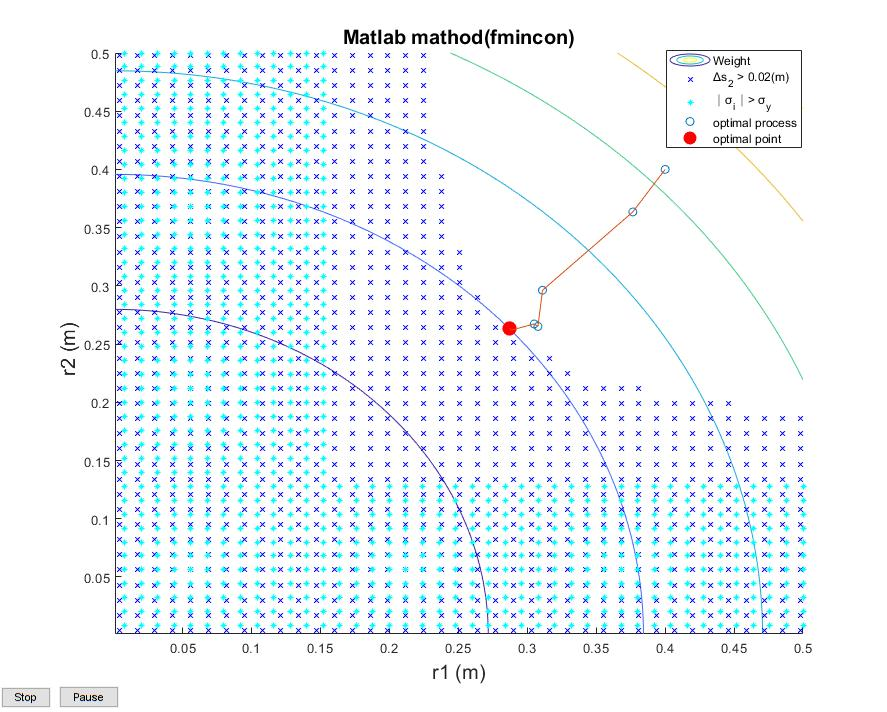
\includegraphics[width=0.6\textwidth]{result.jpg} 
    \caption{10-bar truss 設計空間與收斂路徑} 
    \label{Fig.result} 
\end{figure}

\clearpage
\section{Conclusions}
本次作業主要是根據SOLabNAS的講義 \cite{Chen2017b}所撰寫,可以從結果看出與講義的結果相符。這次作業花了比較多時間在研究LaTex,畢竟之前沒有接觸過這個軟體,
~\\

\section{Appendix}
本作業所有程式碼公佈於軟體原始碼代管服務平台 GitHub,可於下列之 GitHub 網站下載(https://github.com/Chung-Jui/Orientation-Homework.git)。
~\\
\section{References}

\begingroup  % 隱藏預設參考文獻標題
    \renewcommand{\section}[2]{}
    \bibliographystyle{ieeetr}
    \bibliography{ref.bib}
\endgroup

\end{CJK}
\end{document}
